\documentclass{article}

\usepackage{blindtext}
\usepackage{graphicx}
\usepackage{wrapfig}
\usepackage[skip=1ex]{caption}
\usepackage{subcaption}
\usepackage{mdframed}
\usepackage{amsmath}
\usepackage{amsfonts}
\usepackage{amssymb}
\usepackage{amstext}
\usepackage{cancel}
\usepackage{enumitem}
\usepackage[english]{babel}
\usepackage{helvet}
\usepackage{microtype}
\usepackage[pdftex]{hyperref}
\usepackage{float}
\usepackage{nicematrix}
\usepackage{xcolor}
\usepackage{tikz}
\usepackage{geometry}
\geometry{
    a4paper,
    left=2cm,
    right=2cm,
    top=1cm,
    bottom=1cm
}

\special{papersize=8.5in,11in}
\setlength{\pdfpageheight}{\paperheight}
\setlength{\pdfpagewidth}{\paperwidth}

% Macros

% Make inline frac bigger
\newcommand\ifrac[2]{{\displaystyle\frac{#1}{#2}}}

% Aliases
\def\wstar{\overset{*}{\rightharpoonup}}
\def\grad{\nabla}
\def\nt{\notag}
\def\dt{\partial_t}
\def\hal{\ifrac{1}{2}}
\def\ep{\varepsilon}
\def\cK{\mathcal{K}}
\def\cA{\mathcal{A}}
\def\cS{\mathcal{S}}
\def\cV{\mathcal{V}}
\def\Q{\mathbb{Q}}
\def\R{\mathbb{R}}
\def\R{\mathbb{R}}
\def\C{\mathbb{C}}








\begin{document}



\title{Written Assignment 2}

\author{Niraj Venkat}

\date{}

\maketitle

\vspace{.8cm}
\boxed{\text{Exercise} \quad 1}\\\\

\begin{enumerate}[label=(\alph*)]
    \item
    \begin{align*}
        \frac{d}{ds}\,\gamma &= \left(1,2s,3s^2\right) \\
        T(s) &= \frac{1}{\sqrt{9 s^4+4 s^2+1}} \left(1, 2 s, 3 s^2\right) \nt
    \end{align*}


    \item
    \begin{align*} 
        \kappa(s) &= \frac{2}{9 s^4+4 s^2+1} \\
        N(s) &= \frac{1}{\sqrt{(9 s^4+4 s^2+1)(9 s^4+9 s^2+1)}} \left(-9s^3-2s, -9s^4 + 1, 6s^3 + 3s\right)
    \end{align*}

    \item
    \begin{align*}
        B(s) &= \frac{1}{\sqrt{9 s^4+9 s^2+1}} \left(3s^2,-3s,1\right)\\
        \tau(s) &= \frac{3}{9 s^4+9 s^2+1}
    \end{align*}
\end{enumerate}


\vspace{1.8cm}
\boxed{\text{Exercise} \quad 2}\\\\

\begin{enumerate}[label=(\alph*)]
    \item
    The 2-norm of the vector $f(u,v)$ is 1:
    \begin{align*} 
        f(u,v) &= \sqrt{\frac{4 u^2}{\left(u^2+v^2+1\right)^2}+\frac{4 v^2}{\left(u^2+v^2+1\right)^2}+\frac{\left(u^2+v^2-1\right)^2}{\left(u^2+v^2+1\right)^2}}\\
            &= 1
    \end{align*}
    So $f(u,v)$ describes a 2-sphere of radius 1 centered at the origin.

    \item
    Differential $df$ is:
    \begin{align*}
        df &=
        \left(
        \begin{array}{ccc}
        \ifrac{-2 u^2+2 v^2+2}{\left(u^2+v^2+1\right)^2}, & -\ifrac{4 u v}{\left(u^2+v^2+1\right)^2}, & \ifrac{4 u}{\left(u^2+v^2+1\right)^2} \\
        \end{array}
        \right)\, du \\
        &+ 
        \left(
        \begin{array}{ccc}
        -\ifrac{4 u v}{\left(u^2+v^2+1\right)^2}, & \ifrac{2 \left(u^2-v^2+1\right)}{\left(u^2+v^2+1\right)^2}, & \ifrac{4 v}{\left(u^2+v^2+1\right)^2} \\
        \end{array}
        \right)\, dv
    \end{align*}

    \item
    Metric $g$ induced by map $f$ is the first fundamental form $\mathbf{I} = J_f^\texttt{T} \, J_f$:
    $$
        \mathbf{I} =
        \ifrac{4}{\left(u^2+v^2+1\right)^2}
        \left(
        \begin{array}{cc}
        1 & 0 \\
        0 & 1 \\
        \end{array}
        \right)
    $$
    Because our induced metric $\mathbf{I}$ is a positive rescaling of the 2D Euclidean metric we can say that our
    parameterization $f$ is conformal, i.e., $f$ is a conformal map.

    \item
    Gauss map $N$ is $\ifrac{df(\frac{\partial}{\partial u}) \times df(\frac{\partial}{\partial v})}{df(\frac{\partial}{\partial u}) \times df(\frac{\partial}{\partial v})}$:
    \begin{align*}
        N &= \ifrac{1}{\left(u^2+v^2+1\right)} \left(-2 u,-2 v,1-u^2-v^2\right)\\
            &= -f
    \end{align*}
    In our case Gauss map is a constant multiple of the sphere itself.

    \item
    Shape operator $dN$ is:
    \begin{align*}
        dN &= -df\\
            &=
            -\left(
            \begin{array}{ccc}
            \ifrac{-2 u^2+2 v^2+2}{\left(u^2+v^2+1\right)^2}, & -\ifrac{4 u v}{\left(u^2+v^2+1\right)^2}, & \ifrac{4 u}{\left(u^2+v^2+1\right)^2} \\
            \end{array}
            \right)\, du \\
            &-
            \left(
            \begin{array}{ccc}
            -\ifrac{4 u v}{\left(u^2+v^2+1\right)^2}, & \ifrac{2 \left(u^2-v^2+1\right)}{\left(u^2+v^2+1\right)^2}, & \ifrac{4 v}{\left(u^2+v^2+1\right)^2} \\
            \end{array}
            \right)\, dv
    \end{align*}
\end{enumerate}


\vspace{1.8cm}
\boxed{\text{Exercise} \quad 3}\\\\


\begin{enumerate}[label=(\alph*)]
    \item
    Differential $df$ is:
    \begin{align*}
        df &=
        \left(
        \begin{array}{ccc}
        -\sin\theta (r \cos\varphi+R), & \cos\theta (r \cos\varphi+R), & 0 \\
        \end{array}
        \right)\, d\theta \\
        &+ 
        \left(
        \begin{array}{ccc}
        -r \cos\theta \sin\varphi, & -r \sin\theta \sin\varphi, & r \cos\varphi \\
        \end{array}
        \right)\, d\varphi
    \end{align*}

    \item
    Metric $g$ induced by map $f$ is the first fundamental form $\mathbf{I} = J_f^\texttt{T} \, J_f$:
    $$
    \mathbf{I} =
    \left(
    \begin{array}{cc}
    \cos ^2\theta (r \cos \varphi+R)^2+\sin ^2\theta (r \cos \varphi+R)^2 & 0 \\
    0 & r^2 \sin ^2\theta \sin ^2\varphi+r^2 \cos ^2\theta \sin ^2\varphi+r^2 \cos ^2\varphi \\
    \end{array}
    \right)
    $$
    
    \item
    Gauss map $N$ is $\ifrac{df(\frac{\partial}{\partial u}) \times df(\frac{\partial}{\partial v})}{df(\frac{\partial}{\partial u}) \times df(\frac{\partial}{\partial v})}$:
    \begin{align*}
        N = 
        \frac{1}{\sqrt{ \cos \theta \cos^2 \varphi + \cos \varphi \sin^2 \theta + \sin^2 \varphi }}&\Big(\cos \theta \cos \varphi ,
        \sin \theta \cos \varphi ,
        \sin \varphi \Big)
    \end{align*}
    Normals of the torus have no dependence on the radii $r, R$.

    \item
    Shape operator $dN$ is:
    \begin{align*}
        dN &= \frac{1}{\left(\cos (\phi ) \left(\cos (\theta ) \cos (\phi )+\sin ^2(\theta )\right)+\sin ^2(\phi )\right)^{3/2}}\\
            &\Big(
            \frac{-2 \sin (2 \theta ) \cos ^3(\phi )-2 \sin (\theta ) (\cos (\phi )+2 \cos (2 \phi )-\cos (3 \phi )+2)}{8},\\
            &\quad\frac{(\cos (2 \theta )+3) \cos ^3(\phi )+4 \cos (\theta ) \sin ^2(\phi ) \cos (\phi )}{4},\\
            &\quad\frac{\sin (\theta ) \sin (\phi ) \cos (\phi ) (\cos (\phi )-2 \cos (\theta ))}{2}
            \Big)\, du \\
            &+
            \Big(
            -\frac{\cos (\theta ) \left(\sin ^2(\theta ) \sin (2 \phi )+4 \sin (\phi )\right)}{4},\\
            &\quad\quad-\frac{\sin (\theta ) \left(\sin ^2(\theta ) \sin (2 \phi )+4 \sin (\phi )\right)}{4},\\
            &\quad\quad\frac{4 \cos (\theta ) \cos (\phi )+\sin ^2(\theta ) (\cos (2 \phi )+3)}{4}
            \Big)\, dv
    \end{align*}
\end{enumerate}


\pagebreak
\boxed{\text{Exercise} \quad 4}\\\\


Solving the system of equations:
\begin{align*}
    \kappa_1 &= H \pm \sqrt{H^2 - K},\\ \kappa_2 &= H \mp \sqrt{H^2 - K}
\end{align*}

We see that one of these conditions are possible: $\kappa_1 > \kappa_2$, $\kappa_1 < \kappa_2$ or $\kappa_1 = \kappa_2$.\\
The principal curvatures are eigenvalues of the shape operator, and are equal at so called \emph{umbilic points}.


\vspace{1.8cm}
\boxed{\text{Exercise} \quad 5}\\\\


We know that the length of $u$ remains fixed after rotation: $|\mathcal{J}u| = |u|$.\\
Direction of the gradient is the direction of counter-clockwise rotation to increase $\psi$: $\ifrac{\mathcal{J}u}{|\mathcal{J}u|} = \ifrac{\mathcal{J}u}{|u|}$.\\
Lets say we move $u$ in this direction by one unit. To get the magnitude of the gradient, we use the small angle approximation:
$d\psi = \sin(d\psi) = \ifrac{1}{|u|}$.\\
The gradient of $\psi$ with respect to $u$ is: $\grad_u\psi = \ifrac{|\mathcal{J}u|}{|u|^2}$


\vspace{1.8cm}
\boxed{\text{Exercise} \quad 6}\\\\


We can understand this proof by thinking of the point $q$ as being the origin. So shifting the origin around equates to 
rigid motion of the polygon.\\ This would mean different values 
for the cross product of pairs of vectors $(p_i, p_{i+1})$. The sign of $p_i \times p_{i+1}$ depends on the position of $q$.
But excess positive area would cancel out with negative areas.\\
Furthermore Stokes' theorem shows us that the position of $q$ does not matter at all, and we only need the boundary
to describe the area.


\vspace{1.8cm}
\boxed{\text{Exercise} \quad 7}\\\\


Let $X, Y$ be two vectors before immersion. Using the cross product in $\R^3$ we get the area of an infinitesimal patch
of the immersion $f$:
\begin{align*}
    df \wedge df(X, Y) &= df(X) \times df(Y) - df(Y) \times df(X)\\
        &= 2df(X) \times df(Y)\\
        &= 2NdA(X, Y)
\end{align*}
where $dA$ (the area form) is a surface patch and $N$ the normal of that patch (or the Gauss map).\\
If we integrate this over the entire surface $M$, we recover the vector area:
\begin{align*}
    N_{\mathcal{V}} = \int_M NdA &=  \hal \int_M df \wedge df\\
        &= \hal \int_M df \wedge df + (-1) f \wedge d(df) \\
        &= \hal \int_M d(f \wedge df) \tag*{because $d(df) = 0$}\\
        &= \hal \int_{\partial M} f \wedge df \tag*{(using Stokes' thorem)}
\end{align*}


\vspace{1.8cm}
\boxed{\text{Exercise} \quad 8}\\\\


Let $X_1, X_2$ be the principal directions, the eigenvectors of the shape operator.

\begin{align*}
df \wedge dN (X_1, X_2) &= df(X_1) \times dN(X_2) - df(X_2) \times dN(X_1) \\
                        &= df(X_1) \times \kappa_2 df(X_2) - df(X_2) \times \kappa_1 df(X_1) \\
                        &= (\kappa_1 + \kappa_2) \ df(X_1) \times df(X_2) \\
                        &= (\kappa_1 + \kappa_2) N dA(X_1, X_2) \\
                        &= 2H N dA(X_1, X_2)\\\\
dN \wedge dN (X_1, X_2) &= dN(X_1) \times dN(X_2) - dN(X_2) \times dN(X_1) \\
                        &= \kappa_1 df(X_1) \times \kappa_2 df(X_2) - \kappa_2 df(X_2) \times \kappa_1 df(X_1) \\
                        &= (2 \kappa_1 \kappa_2) \ df(X_1) \times df(X_2) \\
                        &= (2 \kappa_1 \kappa_2) N dA(X_1, X_2) \\
                        &= 2K N dA(X_1, X_2)
\end{align*}

We can express any tangent vector $Y$ as a linear combination of the principal directions $X_1$ and $X_2$,
because these directions form an orthonormal basis for the tangent space $T_p M$.
Moreover, the differential is a linear operator. So we conclude that:
\begin{align*}
    df \wedge dN &= 2H N dA\\
    dN \wedge dN &= 2K N dA
\end{align*}


\vspace{1.8cm}
\boxed{\text{Exercise} \quad 9}\\\\


Direction of the gradient is the direction perpendicular to $u$ : $\ifrac{\mathbf{u}^\perp}{|\mathbf{u}^\perp|} = \ifrac{\mathbf{u}^\perp}{|u|}$.\\
Lets say we move $p$ in this direction by one unit. Change in area:
$$dA_\sigma = \hal\,|\mathbf{u}^\perp + 1 - \mathbf{u}^\perp|\, |u| = \hal |u|$$
The gradient of $A_\sigma$ with respect to $p$ is: $\grad_p A_\sigma = \hal \mathbf{u}^\perp$


\vspace{1.8cm}
\boxed{\text{Exercise} \quad 10}\\\\


Volume of a single tet: $\cV = \ifrac13 A h$.\\
Following the same reasoning as the previous exercise, volume gradient for a single tet: $\grad_p \cV =  \ifrac13 A N$\\
where N is the unit normal to the base.\\
For a tet mesh $M$, to express the gradient of the enclosed volume with respect to a given vertex $p$,
we simply sum up the gradients for the tetrahedra containing $p$:
$$
    \grad_p \cV = \sum_i \cV_i = \frac13 \sum_i A_i N_i = \frac13 \int_M NdA = \frac13 N_{\cV}
$$


\pagebreak
\boxed{\text{Exercise} \quad 11}\\\\


Here I reproduce the proof found in the book The Shape of Space by \href{https://www.geometrygames.org/}{Jeffrey Weeks}, and combine it with the concept of \emph{diangles} in the course text.
The book proof uses \emph{lunes}, which have half the area of the diangles. The continuation of a lune is a diangle.\\

We have that a diangle with maximum angle $\pi$ would cover the whole sphere of area $4\pi$.
So a diangle of angle $\alpha$ has area $4\alpha$.\\

Each side of the spherical triangle can be continued into a great circle. Doing this we can construct an \emph{antipodal triangle}, which 
is a mirror image (flipped) version of the triangle on the opposite half of the sphere.\\

For a spherical triangle with area $A$ and interior angles $\alpha_1, \alpha_2, \alpha_3$, we can construct their respective diangles,
with areas $A_1, A_2, A_3$. These diangles overlap both the main and antipodal triangles.\\

\begin{equation*}
    \setlength\arraycolsep{1.5pt}
    \begin{array}{rccccccccccc}
        &\Bigl(\text{\small{Diangle for} $\alpha_1$}\Bigr) &+ &\Bigl(\text{\small{Diangle for} $\alpha_2$}\Bigr) &+ &\Bigl(\text{\small{Diangle for} $\alpha_3$}\Bigr)
        &= &2\Bigl(\text{\small{Main triangle}}\Bigr) &+ &2\Bigl(\text{\small{Antipodal triangle}}\Bigr) &+ &\Bigl(\text{\small{Entire sphere}}\Bigr)\\
        &4\alpha_1 &+ &4\alpha_2 &+ &4\alpha_3 &= &2A &+ &2A &+ &4\pi
    \end{array}
\end{equation*}
$$\implies A = \alpha_1 + \alpha_2 + \alpha_3 - \pi$$


\vspace{1.8cm}
\boxed{\text{Exercise} \quad 12}\\\\

Paraphrasing Weeks:\\
\begin{mdframed}
    The area of any $n$-gon is the sum of the areas of $n-2$ triangles.
    The area of each spherical triangle is the sum of it's angles minus $\pi$.
    Therefore the area of the spherical $n$-gon is the sum of all of the angles minus $(n-2)\pi$.
\end{mdframed}

$$
    A = (2 - n)\pi + \sum_{i=1}^n \beta_i
$$

In general though, for a surface with constant Gaussian curvature $K$ we have:
$$
    KA = (2 - n)\pi + \sum_{i=1}^n \beta_i
$$


\vspace{1.8cm}
\boxed{\text{Exercise} \quad 13}\\\\

As the dihedral angle on the surface approaches $\pi$ by flattening out the star of the vertex $v$,
the area of the spherical polygon approaches zero, because the normals all meet at a sinlge point on the Gauss map.\\
By doing the opposite, the dihedral angles can approach zero or $2\pi$, and the area of the spherical polygon approaches the hemisphere area $2\pi$.
Dihedral angles on the surface become interior angles on the sphere and vice versa.\\
The relationship between the dihedral angle $\theta$ and interior angle $\beta$ can be summarized as $\theta = \pi - \beta$.\\

Alternatively, two adjacent normals $N_i$ and $N_j$ would have a dihedral angle: $\theta = \cos^{-1} \ifrac{N_i \cdot N_i}{|N_i||N_j|}$
which further illustrates this complementary relationship.\\

Using our earlier proof:
\begin{align*}
    A   &= (2 - n)\pi + \sum_{i=1}^n \beta_i \\
        &= (2 - n)\pi + \sum_{i=1}^n (\pi - \theta_i) \\
        &= 2\pi - \sum_{i=1}^n \theta_i \\
        &= d(v)
\end{align*}


\vspace{1.8cm}
\boxed{\text{Exercise} \quad 14}\\\\


A simplicial surface is a triangle mesh, with $n=3$ sides.
Each edge touches two faces, so:
$$\ifrac{nF}{2} = E \implies E = \ifrac{3F}{2}$$
Using our previous result:
\begin{align*}
    \sum_{v \in V} d(v) &= \sum_{v \in V} \Bigl[ 2\pi - \sum_{f \in F_v} \angle_f(v) \Bigr] \\
        &= \sum_{v \in V} 2\pi - \sum_{v \in V} \sum_{f \in F_v} \angle_f(v) \\
        &= 2\pi|V| - \sum_{f \in F} \pi \tag*{\text{(sum of interior angles = $\pi$)}} \\
        &= 2\pi|V| - \pi|F| \\
        &= 2\pi(|V| - \frac{|F|}{2}) \\
        &= 2\pi(|V| + |F| - \frac{3|F|}{2}) \\
        &= 2\pi(|V| - \frac{3|F|}{2} + |F|) \\
        &= 2\pi(|V| - |E| + |F|) \\
        &= 2\pi\chi
\end{align*}
This is just a discrete version of the smooth Gauss-Bonnet theorem which says that the total Gaussian curvature
is always equal to 2$\pi$ times the Euler characteristic.
$$
    \int_M K \, dA = 2\pi\chi
$$
For a surface with boundary, an extra boundary term must be included.\\
For smooth surfaces we integrate geodesic curvature along the boundary, for discrete surfaces we add boundary angle defects.


\pagebreak
\boxed{\text{Exercise} \quad 15}\\\\


Faces add slabs of thickness $r$, hence volume contributed is: $r \sum_{ijk \in F} A_{ijk}$


\vspace{1.8cm}
\boxed{\text{Exercise} \quad 16}\\\\

Cylinders have volume $\pi r^2 L$.\\
Edges add cylindrical wedges of volume $\hal \ell_{ij} \varphi_{ij} r^2$, hence volume contributed is:
$r^2  \sum_{ij \in E} H_{ij}$ where $H_{ij}$ is the total mean curvature for edge $ij$.


\vspace{1.8cm}
\boxed{\text{Exercise} \quad 17}\\\\


Spheres have volume $\frac{4}{3}\pi r^3$.\\
Vertices add spherical cones of volume $\frac{1}{3} \Omega_i r^3$, hence volume contributed is:
$\frac{r^3}{3} \sum_{i \in V} K_i$
because sum of angle defects is equal to sum of Gauss curvature.


\vspace{1.8cm}
\boxed{\text{Exercise} \quad 18}\\\\


Volume of mollified polyhedron is a polynomial in radius $r$:
$$
    \cV(r) = \cV + r \sum_{ijk \in F} A_{ijk} + r^2  \sum_{ij \in E} H_{ij} + \frac{r^3}{3} \sum_{i \in V} K_i
$$

Derivatives w.r.t $r$ give:\\
$$
    \text{volume}_r \overset{\frac{d}{dr}}{\longrightarrow}
    \text{area}_r \overset{\frac{d}{dr}}{\longrightarrow}
    \text{Mean curvature}_r \overset{\frac{d}{dr}}{\longrightarrow}
    \text{Gauss curvature}_r \overset{\frac{d}{dr}}{\longrightarrow} 0
$$


\pagebreak
\boxed{\text{Exercise} \quad 19}\\\\

This uses a proof found in \href{https://www.cs.utexas.edu/users/evouga/uploads/4/5/6/8/45689883/notes3.pdf#page=4}{DDG course by Etienne Vouga}.\\
We have proved that gradient of triangle area is $\grad_{f_i} A_{ijk} = \hal \mathbf{u}_i^\perp$
where vertex $i$ is located at position $f_i$ and
$$\mathbf{u}_i^\perp = \ifrac{f_i - p}{|f_i - p|} (b_1 + b_2)$$

\begin{wrapfigure}{r}{0.3\textwidth}
    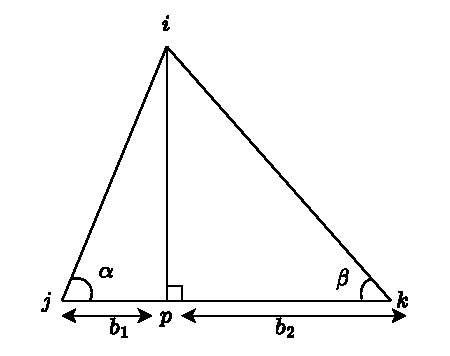
\includegraphics[scale=0.8]{figs/tri.pdf}
\end{wrapfigure}


$p$ can be written as a linear combination: $$p = \ifrac{b_1 f_k + b_2 f_j}{b_1 + b_2}$$

This lets us rewrite the gradient as:
\begin{align*}
    \grad_{f_i} A_{ijk} &= \hal \mathbf{u}_i^\perp\\
        &= \hal \ifrac{f_i - p}{|f_i - p|} (b_1 + b_2)\\
        &= \hal \ifrac{f_i - \Big(\ifrac{b_1 f_k + b_2 f_j}{b_1 + b_2}\Big)}{|f_i - p|} (b_1 + b_2)   \tag*{\text{(substituting $p$)}}\\
        &= \hal \ifrac{b_1 f_i + b_2 f_i - b_1 f_k - b_2 f_j}{|f_i - p|} \\
        &= \hal \Bigl[\frac{b_1}{|f_i - p|} (f_i - f_k) + \frac{b_2}{|f_i - p|} (f_i - f_j)\Bigr] \\
        &= \hal \Bigl[\cot(\angle ijp) (f_i - f_k) + \cot(\angle ikp) (f_i - f_j)\Bigr] \\
        &= \hal \Bigl[\cot(\alpha_{ip}) (f_i - f_k) + \cot(\beta_{ip}) (f_i - f_j)\Bigr] \\
\end{align*}

Now we express the gradient of total surface area expressed in terms of edges $ij$ oriented from $i \rightarrow j$.\\
The label $p$ in our diagram we now call $j$ when referring to edges:
\begin{align*}
    \grad_{f_i} \sum_{ijk \in F} A_{ijk} &= \hal \sum_{ij \in E}  \mathbf{u}_i^\perp -  \mathbf{u}_j^\perp\\
        &= \hal \sum_{ij \in E} \cot(\alpha_{ij}) + \cot(\beta_{ij}) (f_i - f_j)
\end{align*}


\vspace{1.8cm}
\boxed{\text{Exercise} \quad 20}\\\\


Gradient of the total discrete scalar mean curvature gives:
\begin{align*}
    \nabla_{f_i} \hal \sum_{ij \in E} \theta_{ij} l_{ij} &= \hal \sum_{ij \in E} \cancelto{0}{(\nabla_{f_i} \theta_{ij}) l_{ij}} + \theta_{ij} (\nabla_{f_i} l_{ij}) \tag*{\text{(product rule)}}\\
        &= \hal \sum_{ij \in E} \theta_{ij} (\nabla_{f_i} l_{ij}) \tag*{using Schläfli formula: $(\nabla_{f_i} \theta_{ij}) l_{ij} = 0$}\\
        &= \hal \sum_{ij \in E} \theta_{ij} \frac{f_j - f_i}{l_{ij}} \\
        &= \hal \sum_{ij \in E} \frac{\theta_{ij}}{l_{ij}} (f_j - f_i) \\
        &= K N_i
\end{align*}

Equates to sum of the Gauss curvature normals over the dual cell of vertex $i$.


\vspace{1.8cm}
\boxed{\text{Exercise} \quad 21}\\\\


The gradient of the total discrete scalar Gauss curvature is zero, because the sum of Gauss curvatures $K_i$ is 
the sum of angle defects $d(v)$, and by Gauss-Bonnet theorem results in a constant multiple of the Euler characteristic $\chi$.\\\\
$\chi = (2 - 2g)$ is a topological invariant that does not change unless we change the genus of the surface,
or change the number of mesh elements in a way that changes $\chi$: $|V|, |E|, |F|$. 
Another way of stating this result is that the gradient of $\sum_i K_i$ w.r.t motion of any vertex $i$ is zero.

$$
\nabla_{f_i} \sum_{\ell \in V} \Bigl[2\pi - \sum_{jk\ell \in F} \varphi^{jk}\Bigr]
= 2\pi \nabla_{f_i}\chi
= 0
$$    






























\end{document}
